% Name: Moore machine
% Description: The 101 detector as a Moore machine: the output belongs to the state, so a fourth state S3 is needed to output the 1.
% Tags: Moore machine, sequence detector, finite state machine, transducer

\usetikzlibrary{automata, arrows.meta}

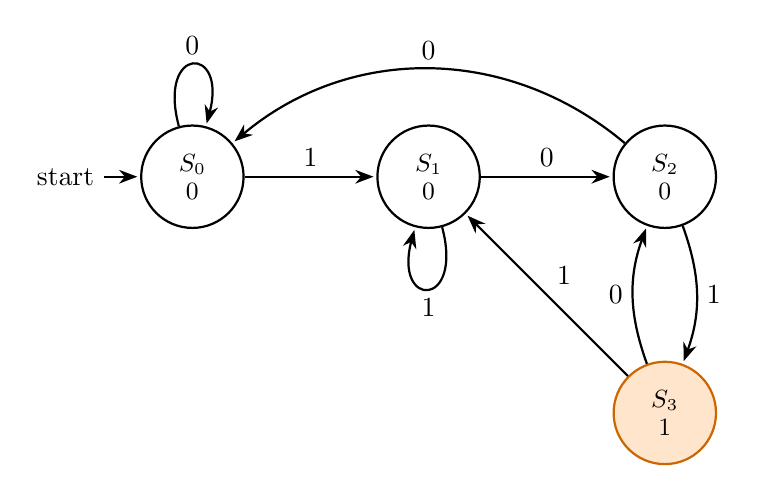
\begin{tikzpicture}[shorten >=1pt, auto, thick, >={Stealth},
    every state/.style={minimum size=13mm, font=\small, align=center, inner sep=1pt}]
  % Each state shows its name over its output.
  \node[state, initial] (s0) at (0,0) {$S_0$\\[-1pt]$0$};
  \node[state] (s1) at (3,0) {$S_1$\\[-1pt]$0$};
  \node[state] (s2) at (6,0) {$S_2$\\[-1pt]$0$};
  \node[state, fill=orange!20, draw=orange!80!black] (s3) at (6,-3) {$S_3$\\[-1pt]$1$};
  \path[->]
    (s0) edge[loop above] node {$0$} ()
         edge node {$1$} (s1)
    (s1) edge[loop below] node {$1$} ()
         edge node {$0$} (s2)
    (s2) edge[bend right=40, swap] node {$0$} (s0)
         edge[bend left=20] node {$1$} (s3)
    (s3) edge[swap] node {$1$} (s1)
         edge[bend left=20] node {$0$} (s2);
\end{tikzpicture}
